\documentclass[twoside]{book}

% Packages required by doxygen
\usepackage{fixltx2e}
\usepackage{calc}
\usepackage{doxygen}
\usepackage[export]{adjustbox} % also loads graphicx
\usepackage{graphicx}
\usepackage[utf8]{inputenc}
\usepackage{makeidx}
\usepackage{multicol}
\usepackage{multirow}
\PassOptionsToPackage{warn}{textcomp}
\usepackage{textcomp}
\usepackage[nointegrals]{wasysym}
\usepackage[table]{xcolor}

% Font selection
\usepackage[T1]{fontenc}
\usepackage[scaled=.90]{helvet}
\usepackage{courier}
\usepackage{amssymb}
\usepackage{sectsty}
\renewcommand{\familydefault}{\sfdefault}
\allsectionsfont{%
  \fontseries{bc}\selectfont%
  \color{darkgray}%
}
\renewcommand{\DoxyLabelFont}{%
  \fontseries{bc}\selectfont%
  \color{darkgray}%
}
\newcommand{\+}{\discretionary{\mbox{\scriptsize$\hookleftarrow$}}{}{}}

% Page & text layout
\usepackage{geometry}
\geometry{%
  a4paper,%
  top=2.5cm,%
  bottom=2.5cm,%
  left=2.5cm,%
  right=2.5cm%
}
\tolerance=750
\hfuzz=15pt
\hbadness=750
\setlength{\emergencystretch}{15pt}
\setlength{\parindent}{0cm}
\setlength{\parskip}{3ex plus 2ex minus 2ex}
\makeatletter
\renewcommand{\paragraph}{%
  \@startsection{paragraph}{4}{0ex}{-1.0ex}{1.0ex}{%
    \normalfont\normalsize\bfseries\SS@parafont%
  }%
}
\renewcommand{\subparagraph}{%
  \@startsection{subparagraph}{5}{0ex}{-1.0ex}{1.0ex}{%
    \normalfont\normalsize\bfseries\SS@subparafont%
  }%
}
\makeatother

% Headers & footers
\usepackage{fancyhdr}
\pagestyle{fancyplain}
\fancyhead[LE]{\fancyplain{}{\bfseries\thepage}}
\fancyhead[CE]{\fancyplain{}{}}
\fancyhead[RE]{\fancyplain{}{\bfseries\leftmark}}
\fancyhead[LO]{\fancyplain{}{\bfseries\rightmark}}
\fancyhead[CO]{\fancyplain{}{}}
\fancyhead[RO]{\fancyplain{}{\bfseries\thepage}}
\fancyfoot[LE]{\fancyplain{}{}}
\fancyfoot[CE]{\fancyplain{}{}}
\fancyfoot[RE]{\fancyplain{}{\bfseries\scriptsize Generated by Doxygen }}
\fancyfoot[LO]{\fancyplain{}{\bfseries\scriptsize Generated by Doxygen }}
\fancyfoot[CO]{\fancyplain{}{}}
\fancyfoot[RO]{\fancyplain{}{}}
\renewcommand{\footrulewidth}{0.4pt}
\renewcommand{\chaptermark}[1]{%
  \markboth{#1}{}%
}
\renewcommand{\sectionmark}[1]{%
  \markright{\thesection\ #1}%
}

% Indices & bibliography
\usepackage{natbib}
\usepackage[titles]{tocloft}
\setcounter{tocdepth}{3}
\setcounter{secnumdepth}{5}
\makeindex

% Hyperlinks (required, but should be loaded last)
\usepackage{ifpdf}
\ifpdf
  \usepackage[pdftex,pagebackref=true]{hyperref}
\else
  \usepackage[ps2pdf,pagebackref=true]{hyperref}
\fi
\hypersetup{%
  colorlinks=true,%
  linkcolor=blue,%
  citecolor=blue,%
  unicode%
}

% Custom commands
\newcommand{\clearemptydoublepage}{%
  \newpage{\pagestyle{empty}\cleardoublepage}%
}

\usepackage{caption}
\captionsetup{labelsep=space,justification=centering,font={bf},singlelinecheck=off,skip=4pt,position=top}

%===== C O N T E N T S =====

\begin{document}

% Titlepage & ToC
\hypersetup{pageanchor=false,
             bookmarksnumbered=true,
             pdfencoding=unicode
            }
\pagenumbering{alph}
\begin{titlepage}
\vspace*{7cm}
\begin{center}%
{\Large My Project }\\
\vspace*{1cm}
{\large Generated by Doxygen 1.8.13}\\
\end{center}
\end{titlepage}
\clearemptydoublepage
\pagenumbering{roman}
\tableofcontents
\clearemptydoublepage
\pagenumbering{arabic}
\hypersetup{pageanchor=true}

%--- Begin generated contents ---
\chapter{Hierarchical Index}
\section{Class Hierarchy}
This inheritance list is sorted roughly, but not completely, alphabetically\+:\begin{DoxyCompactList}
\item \contentsline{section}{Main}{\pageref{classMain}}{}
\item \contentsline{section}{Mundo}{\pageref{classMundo}}{}
\item \contentsline{section}{Veiculo}{\pageref{classVeiculo}}{}
\begin{DoxyCompactList}
\item \contentsline{section}{Caminhao}{\pageref{classCaminhao}}{}
\item \contentsline{section}{Carro}{\pageref{classCarro}}{}
\item \contentsline{section}{Moto}{\pageref{classMoto}}{}
\end{DoxyCompactList}
\end{DoxyCompactList}

\chapter{Class Index}
\section{Class List}
Here are the classes, structs, unions and interfaces with brief descriptions\+:\begin{DoxyCompactList}
\item\contentsline{section}{\hyperlink{classCaminhao}{Caminhao} }{\pageref{classCaminhao}}{}
\item\contentsline{section}{\hyperlink{classCarro}{Carro} }{\pageref{classCarro}}{}
\item\contentsline{section}{\hyperlink{classMain}{Main} }{\pageref{classMain}}{}
\item\contentsline{section}{\hyperlink{classMoto}{Moto} }{\pageref{classMoto}}{}
\item\contentsline{section}{\hyperlink{classMundo}{Mundo} }{\pageref{classMundo}}{}
\item\contentsline{section}{\hyperlink{classVeiculo}{Veiculo} }{\pageref{classVeiculo}}{}
\end{DoxyCompactList}

\chapter{Class Documentation}
\hypertarget{classCaminhao}{}\section{Caminhao Class Reference}
\label{classCaminhao}\index{Caminhao@{Caminhao}}


Inheritance diagram for Caminhao\+:

\hypertarget{classCarro}{}\section{Carro Class Reference}
\label{classCarro}\index{Carro@{Carro}}


Inheritance diagram for Carro\+:
% FIG 0


Collaboration diagram for Carro\+:
% FIG 1
\subsection*{Public Member Functions}
\begin{DoxyCompactItemize}
\item 
\mbox{\Hypertarget{classCarro_a04825b53411fbe9dc67f52147d06cda0}\label{classCarro_a04825b53411fbe9dc67f52147d06cda0}} 
{\bfseries Carro} (int x, int y, int velocidade, String cor)
\item 
\mbox{\Hypertarget{classCarro_ac1474da2f7b971afe6c865f896287d5a}\label{classCarro_ac1474da2f7b971afe6c865f896287d5a}} 
void {\bfseries move} ()
\end{DoxyCompactItemize}
\subsection*{Public Attributes}
\begin{DoxyCompactItemize}
\item 
\mbox{\Hypertarget{classCarro_affc88d52cea6659e1d2cd57e43a12701}\label{classCarro_affc88d52cea6659e1d2cd57e43a12701}} 
int {\bfseries mov} = r.\+next\+Int(4)
\end{DoxyCompactItemize}


The documentation for this class was generated from the following file\+:\begin{DoxyCompactItemize}
\item 
Carro.\+java\end{DoxyCompactItemize}

\hypertarget{classMain}{}\section{Main Class Reference}
\label{classMain}\index{Main@{Main}}
\subsection*{Static Public Member Functions}
\begin{DoxyCompactItemize}
\item 
\mbox{\Hypertarget{classMain_a8a5d0f827edddff706cc0e6740d0579a}\label{classMain_a8a5d0f827edddff706cc0e6740d0579a}} 
static void {\bfseries main} (String\mbox{[}$\,$\mbox{]} args)  throws Interrupted\+Exception 
\end{DoxyCompactItemize}


\subsection{Detailed Description}
\begin{DoxyAuthor}{Author}
Victor 
\end{DoxyAuthor}


The documentation for this class was generated from the following file\+:\begin{DoxyCompactItemize}
\item 
Main.\+java\end{DoxyCompactItemize}

\hypertarget{classMoto}{}\section{Moto Class Reference}
\label{classMoto}\index{Moto@{Moto}}


Inheritance diagram for Moto\+:\nopagebreak
\begin{figure}[H]
\begin{center}
\leavevmode
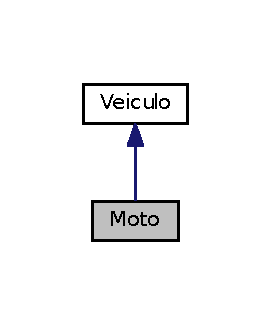
\includegraphics[width=130pt]{classMoto__inherit__graph}
\end{center}
\end{figure}


Collaboration diagram for Moto\+:\nopagebreak
\begin{figure}[H]
\begin{center}
\leavevmode
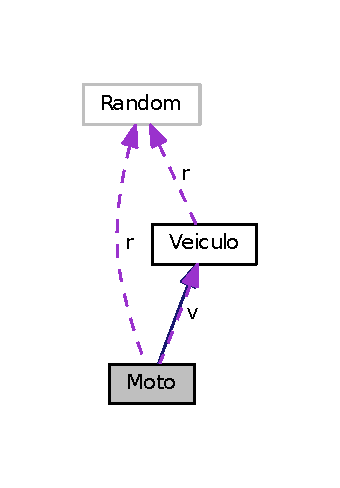
\includegraphics[width=163pt]{classMoto__coll__graph}
\end{center}
\end{figure}
\subsection*{Public Member Functions}
\begin{DoxyCompactItemize}
\item 
\hyperlink{classMoto_a676b8823dfda966d8a40d6624c5169b6}{Moto} (int x, int y, int velocidade, String cor, boolean fabrica)
\item 
void \hyperlink{classMoto_a161a14fdc1ead9e078b37537a61bc199}{move} (\hyperlink{classMoto}{Moto} m)
\item 
int \hyperlink{classMoto_a56bf604e45484d316f4a472254370289}{verificaX} (int x)
\item 
int \hyperlink{classMoto_a6933149c85bd01bad40a0e4e0052a430}{verificaY} (int y)
\end{DoxyCompactItemize}


\subsection{Constructor \& Destructor Documentation}
\mbox{\Hypertarget{classMoto_a676b8823dfda966d8a40d6624c5169b6}\label{classMoto_a676b8823dfda966d8a40d6624c5169b6}} 
\index{Moto@{Moto}!Moto@{Moto}}
\index{Moto@{Moto}!Moto@{Moto}}
\subsubsection{\texorpdfstring{Moto()}{Moto()}}
{\footnotesize\ttfamily Moto.\+Moto (\begin{DoxyParamCaption}\item[{int}]{x,  }\item[{int}]{y,  }\item[{int}]{velocidade,  }\item[{String}]{cor,  }\item[{boolean}]{fabrica }\end{DoxyParamCaption})\hspace{0.3cm}{\ttfamily [inline]}}

Construtor da classe \hyperlink{classMoto}{Moto}, que usa um super para chamar o construtor da classe Veículo

\begin{DoxySeeAlso}{See also}
\hyperlink{classVeiculo}{Veiculo} 
\end{DoxySeeAlso}

\begin{DoxyParams}{Parameters}
{\em x} & \\
\hline
{\em y} & \\
\hline
{\em velocidade} & \\
\hline
{\em cor} & \\
\hline
{\em fabrica} & \\
\hline
\end{DoxyParams}


\subsection{Member Function Documentation}
\mbox{\Hypertarget{classMoto_a161a14fdc1ead9e078b37537a61bc199}\label{classMoto_a161a14fdc1ead9e078b37537a61bc199}} 
\index{Moto@{Moto}!move@{move}}
\index{move@{move}!Moto@{Moto}}
\subsubsection{\texorpdfstring{move()}{move()}}
{\footnotesize\ttfamily void Moto.\+move (\begin{DoxyParamCaption}\item[{\hyperlink{classMoto}{Moto}}]{m }\end{DoxyParamCaption})\hspace{0.3cm}{\ttfamily [inline]}}

Função que movimenta a moto, recebendo um objeto da própria classe como parâmetro 
\begin{DoxyParams}{Parameters}
{\em m} & \\
\hline
\end{DoxyParams}
Gerando um número aleatório para movimentação do veículo em 4 direções possíveis

Ifs para verificação do resultado obtido no random\mbox{\Hypertarget{classMoto_a56bf604e45484d316f4a472254370289}\label{classMoto_a56bf604e45484d316f4a472254370289}} 
\index{Moto@{Moto}!verificaX@{verificaX}}
\index{verificaX@{verificaX}!Moto@{Moto}}
\subsubsection{\texorpdfstring{verifica\+X()}{verificaX()}}
{\footnotesize\ttfamily int Moto.\+verificaX (\begin{DoxyParamCaption}\item[{int}]{x }\end{DoxyParamCaption})\hspace{0.3cm}{\ttfamily [inline]}}

Função que verifica se a moto chegou ao limite do mapa em X e reseta a coordenada 
\begin{DoxyParams}{Parameters}
{\em x} & \\
\hline
\end{DoxyParams}
\begin{DoxyReturn}{Returns}

\end{DoxyReturn}
\mbox{\Hypertarget{classMoto_a6933149c85bd01bad40a0e4e0052a430}\label{classMoto_a6933149c85bd01bad40a0e4e0052a430}} 
\index{Moto@{Moto}!verificaY@{verificaY}}
\index{verificaY@{verificaY}!Moto@{Moto}}
\subsubsection{\texorpdfstring{verifica\+Y()}{verificaY()}}
{\footnotesize\ttfamily int Moto.\+verificaY (\begin{DoxyParamCaption}\item[{int}]{y }\end{DoxyParamCaption})\hspace{0.3cm}{\ttfamily [inline]}}

Função que verifica se a moto chegou ao limite do mapa em Y e reseta a coordenada 
\begin{DoxyParams}{Parameters}
{\em y} & \\
\hline
\end{DoxyParams}
\begin{DoxyReturn}{Returns}

\end{DoxyReturn}


The documentation for this class was generated from the following file\+:\begin{DoxyCompactItemize}
\item 
Moto.\+java\end{DoxyCompactItemize}

\hypertarget{classMundo}{}\section{Mundo Class Reference}
\label{classMundo}\index{Mundo@{Mundo}}


Collaboration diagram for Mundo\+:\nopagebreak
\begin{figure}[H]
\begin{center}
\leavevmode
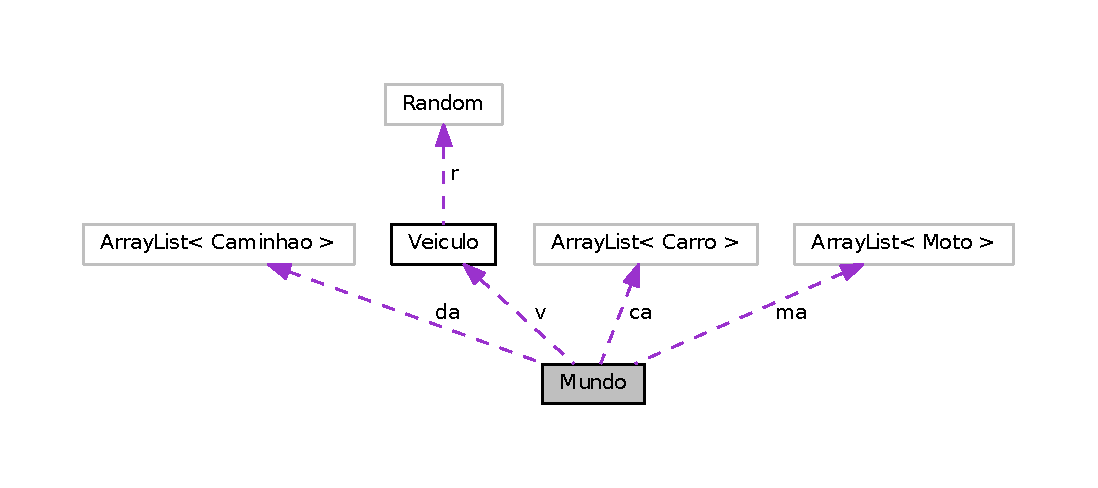
\includegraphics[width=350pt]{classMundo__coll__graph}
\end{center}
\end{figure}
\subsection*{Public Member Functions}
\begin{DoxyCompactItemize}
\item 
void \hyperlink{classMundo_a6793ddedae676faa577ac3545dc4a190}{gera\+Veiculos} ()
\item 
void \hyperlink{classMundo_a500511141a45b1b95301612109703f02}{refaz\+Mapa} ()
\item 
void \hyperlink{classMundo_adbafcb32f5f209eda97e1c7953c6e599}{desenha\+Mundo} ()
\item 
void \hyperlink{classMundo_ab2de7a750f9e410a7e10ac707b5bf500}{atualiza\+Mundo} ()
\item 
void \hyperlink{classMundo_ac5525a65a2bc9c8b333c6594aa9503ca}{detecta\+Colisao} ()
\item 
void \hyperlink{classMundo_a96be554c9f3734a55b27b10bae5f6527}{gera\+Veiculo} ()
\end{DoxyCompactItemize}
\subsection*{Public Attributes}
\begin{DoxyCompactItemize}
\item 
int {\bfseries mapa} \mbox{[}$\,$\mbox{]}\mbox{[}$\,$\mbox{]}
\end{DoxyCompactItemize}


\subsection{Member Function Documentation}
\mbox{\Hypertarget{classMundo_ab2de7a750f9e410a7e10ac707b5bf500}\label{classMundo_ab2de7a750f9e410a7e10ac707b5bf500}} 
\index{Mundo@{Mundo}!atualiza\+Mundo@{atualiza\+Mundo}}
\index{atualiza\+Mundo@{atualiza\+Mundo}!Mundo@{Mundo}}
\subsubsection{\texorpdfstring{atualiza\+Mundo()}{atualizaMundo()}}
{\footnotesize\ttfamily void Mundo.\+atualiza\+Mundo (\begin{DoxyParamCaption}{ }\end{DoxyParamCaption})\hspace{0.3cm}{\ttfamily [inline]}}

Função que atualiza o mundo fazendo os veículos se moverem \mbox{\Hypertarget{classMundo_adbafcb32f5f209eda97e1c7953c6e599}\label{classMundo_adbafcb32f5f209eda97e1c7953c6e599}} 
\index{Mundo@{Mundo}!desenha\+Mundo@{desenha\+Mundo}}
\index{desenha\+Mundo@{desenha\+Mundo}!Mundo@{Mundo}}
\subsubsection{\texorpdfstring{desenha\+Mundo()}{desenhaMundo()}}
{\footnotesize\ttfamily void Mundo.\+desenha\+Mundo (\begin{DoxyParamCaption}{ }\end{DoxyParamCaption})\hspace{0.3cm}{\ttfamily [inline]}}

Função que desenha o mundo Contadores para exibir quantidade de veículos

Desenhando o mapa com base no que foi refeito

Imprimindo a legenda

Contadores de veículos\mbox{\Hypertarget{classMundo_ac5525a65a2bc9c8b333c6594aa9503ca}\label{classMundo_ac5525a65a2bc9c8b333c6594aa9503ca}} 
\index{Mundo@{Mundo}!detecta\+Colisao@{detecta\+Colisao}}
\index{detecta\+Colisao@{detecta\+Colisao}!Mundo@{Mundo}}
\subsubsection{\texorpdfstring{detecta\+Colisao()}{detectaColisao()}}
{\footnotesize\ttfamily void Mundo.\+detecta\+Colisao (\begin{DoxyParamCaption}{ }\end{DoxyParamCaption})\hspace{0.3cm}{\ttfamily [inline]}}

Função que detecta colisão Colisão entre carros apenas

Essa parte verifica se o veículo é ele mesmo, e não o remove

Colisão entre caminhões apenas

Colisão entre motos apenas

Colisão entre caminhão e carro

Colisão entre caminhão e moto

Colisão entre carro e moto \mbox{\Hypertarget{classMundo_a96be554c9f3734a55b27b10bae5f6527}\label{classMundo_a96be554c9f3734a55b27b10bae5f6527}} 
\index{Mundo@{Mundo}!gera\+Veiculo@{gera\+Veiculo}}
\index{gera\+Veiculo@{gera\+Veiculo}!Mundo@{Mundo}}
\subsubsection{\texorpdfstring{gera\+Veiculo()}{geraVeiculo()}}
{\footnotesize\ttfamily void Mundo.\+gera\+Veiculo (\begin{DoxyParamCaption}{ }\end{DoxyParamCaption})\hspace{0.3cm}{\ttfamily [inline]}}

Função que gera um veículo se passarem em fábricas Já que o veículo passou numa fábrica, ele fica impossibilitado de gerar novamente caso não saia da fabrica \mbox{\Hypertarget{classMundo_a6793ddedae676faa577ac3545dc4a190}\label{classMundo_a6793ddedae676faa577ac3545dc4a190}} 
\index{Mundo@{Mundo}!gera\+Veiculos@{gera\+Veiculos}}
\index{gera\+Veiculos@{gera\+Veiculos}!Mundo@{Mundo}}
\subsubsection{\texorpdfstring{gera\+Veiculos()}{geraVeiculos()}}
{\footnotesize\ttfamily void Mundo.\+gera\+Veiculos (\begin{DoxyParamCaption}{ }\end{DoxyParamCaption})\hspace{0.3cm}{\ttfamily [inline]}}

Função que gera veículos aleatóriamente $<$ Verificando se o carro foi gerado onde há uma fábrica, se sim, trocando-\/o \mbox{\Hypertarget{classMundo_a500511141a45b1b95301612109703f02}\label{classMundo_a500511141a45b1b95301612109703f02}} 
\index{Mundo@{Mundo}!refaz\+Mapa@{refaz\+Mapa}}
\index{refaz\+Mapa@{refaz\+Mapa}!Mundo@{Mundo}}
\subsubsection{\texorpdfstring{refaz\+Mapa()}{refazMapa()}}
{\footnotesize\ttfamily void Mundo.\+refaz\+Mapa (\begin{DoxyParamCaption}{ }\end{DoxyParamCaption})\hspace{0.3cm}{\ttfamily [inline]}}

Função que zera o mapa, acabando com o rastro que ficaria caso o mapa não fosse zerado Esse é um comentário a parte, mas que achei legal estar na documentação\+: Parte do código que alteraria a situação de um veículo que não está mais em uma fábrica para false Essa parte foi comentada porém não removida pois faz a quantidade de veículos aumentar ao invés de zerar, como no vídeo de exemplo Apesar de ser o mais lógico colocar um veículo fora de uma fábrica como false, decidi remover do código final Removi pois o funcionamento do vídeo de exemplo se asemelha mais com o código funcionando sem essa parte

for(int a = 0; a $<$ ca.\+size(); a++) \{ int xa = ca.\+get(a).get\+X(); int ya = ca.\+get(a).get\+Y(); for(int i = 0; i$<$30; i++) \{ for(int j = 0; j $<$ 60; j++) \{ if(i == xa \&\& j == ya) \{ if(mapa\mbox{[}i\mbox{]}\mbox{[}j\mbox{]} != 2 \&\& ca.\+get(a).get\+Fabrica() == true) \{ ca.\+get(a).set\+Fabrica(false); \} \} \} \} \}

for(int a = 0; a $<$ da.\+size(); a++) \{ int xa = da.\+get(a).get\+X(); int ya = da.\+get(a).get\+Y(); for(int i = 0; i$<$30; i++) \{ for(int j = 0; j $<$ 60; j++) \{ if(i == xa \&\& j == ya) \{ if(mapa\mbox{[}i\mbox{]}\mbox{[}j\mbox{]} != 2 \&\& da.\+get(a).get\+Fabrica() == true) \{ da.\+get(a).set\+Fabrica(false); \} \} \} \} \}

for(int a = 0; a $<$ da.\+size(); a++) \{ int xa = da.\+get(a).get\+X(); int ya = da.\+get(a).get\+Y(); for(int i = 0; i$<$30; i++) \{ for(int j = 0; j $<$ 60; j++) \{ if(i == xa \&\& j == ya) \{ if(mapa\mbox{[}i\mbox{]}\mbox{[}j\mbox{]} != 2 \&\& da.\+get(a).get\+Fabrica() == true) \{ da.\+get(a).set\+Fabrica(false); \} \} \} \} \}

Adicionando os novos veículos no mapa

Obtendo as corrdenadas do veículo

S\+Obrescrevendo 2 caso seja uma fábrica 

\subsection{Member Data Documentation}
\mbox{\Hypertarget{classMundo_a8332b2d52b9f317338a4d6cbe10bbcbb}\label{classMundo_a8332b2d52b9f317338a4d6cbe10bbcbb}} 
\index{Mundo@{Mundo}!mapa@{mapa}}
\index{mapa@{mapa}!Mundo@{Mundo}}
\subsubsection{\texorpdfstring{mapa}{mapa}}
{\footnotesize\ttfamily int Mundo.\+mapa\mbox{[}$\,$\mbox{]}\mbox{[}$\,$\mbox{]}}

{\bfseries Initial value\+:}
\begin{DoxyCode}
= \{\{1,1,1,1,1,1,1,1,1,1,1,1,1,1,1,1,1,1,1,1,1,1,1,1,1,1,1,1,1,1,1,1,1,1,1,1,1,1,1,1,1,1,1,1,1,1,1,1,1,1,1,1
      ,1,1,1,1,1,1,1,1\},
                            \{1,0,0,0,0,0,0,0,0,0,0,0,0,0,0,0,0,0,0,0,0,0,0,0,0,0,0,0,0,0,0,0,0,0,0,0,0,0,0,
      0,0,0,0,0,0,0,0,0,0,0,0,0,0,0,0,0,0,0,0,1\},
                            \{1,0,0,0,0,0,0,0,0,0,0,0,0,0,0,0,0,0,0,0,0,0,0,0,0,0,0,0,0,0,0,0,0,0,0,0,0,0,0,
      0,0,0,0,0,0,0,0,0,0,0,0,0,0,0,0,0,0,0,0,1\},
                            \{1,0,0,0,0,0,0,0,0,0,0,0,0,0,0,0,0,0,0,0,0,0,0,0,0,0,0,0,0,0,0,0,0,0,0,0,0,0,0,
      0,0,0,0,0,0,0,0,0,0,0,0,0,0,0,0,0,0,0,0,1\},
                            \{1,0,0,0,0,2,2,2,2,2,0,0,0,0,0,0,0,0,0,0,0,0,0,0,0,0,0,0,0,0,0,0,0,0,0,0,0,0,0,
      0,0,0,0,2,2,2,2,2,0,0,0,0,0,0,0,0,0,0,0,1\},
                            \{1,0,0,0,0,2,2,2,2,2,0,0,0,0,0,0,0,0,0,0,0,0,0,0,0,0,0,0,0,0,0,0,0,0,0,0,0,0,0,
      0,0,0,0,2,2,2,2,2,0,0,0,0,0,0,0,0,0,0,0,1\},
                            \{1,0,0,0,0,2,2,2,2,2,0,0,0,0,0,0,0,0,0,0,0,0,0,0,0,0,0,0,0,0,0,0,0,0,0,0,0,0,0,
      0,0,0,0,2,2,2,2,2,0,0,0,0,0,0,0,0,0,0,0,1\},
                            \{1,0,0,0,0,0,0,0,0,0,0,0,0,0,0,0,0,0,0,0,0,0,0,0,0,0,0,0,0,0,0,0,0,0,0,0,0,0,0,
      0,0,0,0,0,0,0,0,0,0,0,0,0,0,0,0,0,0,0,0,1\},
                            \{1,0,0,0,0,0,0,0,0,0,0,0,0,0,0,0,0,0,0,0,0,0,0,0,0,0,0,0,0,0,0,0,0,0,0,0,0,0,0,
      0,0,0,0,0,0,0,0,0,0,0,0,0,0,0,0,0,0,0,0,1\},
                            \{1,0,0,0,0,0,0,0,0,0,0,0,0,0,0,0,0,0,0,0,0,0,0,0,0,0,0,0,0,0,0,0,0,0,0,0,0,0,0,
      0,0,0,0,0,0,0,0,0,0,0,0,0,0,0,0,0,0,0,0,1\},
                            \{1,0,0,0,0,0,0,0,0,0,0,0,0,0,0,0,0,0,0,0,0,0,0,0,0,0,0,0,0,0,0,0,0,0,0,0,0,0,0,
      0,0,0,0,0,0,0,0,0,0,0,0,0,0,0,0,0,0,0,0,1\},
                            \{1,0,0,0,0,0,0,0,0,0,0,0,0,0,0,0,0,0,0,0,0,0,0,0,0,0,0,0,0,0,0,0,0,0,0,0,0,0,0,
      0,0,0,0,0,0,0,0,0,0,0,0,0,0,0,0,0,0,0,0,1\},
                            \{1,0,0,0,0,0,0,0,0,0,0,0,0,0,0,0,0,0,0,0,0,0,0,0,0,0,0,0,0,0,0,0,0,0,0,0,0,0,0,
      0,0,0,0,0,0,0,0,0,0,0,0,0,0,0,0,0,0,0,0,1\},
                            \{1,0,0,0,0,0,0,0,0,0,0,0,0,0,0,0,0,0,0,0,0,0,0,0,0,0,2,2,2,2,2,2,2,0,0,0,0,0,0,
      0,0,0,0,0,0,0,0,0,0,0,0,0,0,0,0,0,0,0,0,1\},
                            \{1,0,0,0,0,0,0,0,0,0,0,0,0,0,0,0,0,0,0,0,0,0,0,0,0,0,2,2,2,2,2,2,2,0,0,0,0,0,0,
      0,0,0,0,0,0,0,0,0,0,0,0,0,0,0,0,0,0,0,0,1\},
                            \{1,0,0,0,0,0,0,0,0,0,0,0,0,0,0,0,0,0,0,0,0,0,0,0,0,0,2,2,2,2,2,2,2,0,0,0,0,0,0,
      0,0,0,0,0,0,0,0,0,0,0,0,0,0,0,0,0,0,0,0,1\},
                            \{1,0,0,0,0,0,0,0,0,0,0,0,0,0,0,0,0,0,0,0,0,0,0,0,0,0,0,0,0,0,0,0,0,0,0,0,0,0,0,
      0,0,0,0,0,0,0,0,0,0,0,0,0,0,0,0,0,0,0,0,1\},
                            \{1,0,0,0,0,0,0,0,0,0,0,0,0,0,0,0,0,0,0,0,0,0,0,0,0,0,0,0,0,0,0,0,0,0,0,0,0,0,0,
      0,0,0,0,0,0,0,0,0,0,0,0,0,0,0,0,0,0,0,0,1\},
                            \{1,0,0,0,0,0,0,0,0,0,0,0,0,0,0,0,0,0,0,0,0,0,0,0,0,0,0,0,0,0,0,0,0,0,0,0,0,0,0,
      0,0,0,0,0,0,0,0,0,0,0,0,0,0,0,0,0,0,0,0,1\},
                            \{1,0,0,0,0,0,0,0,0,0,0,0,0,0,0,0,0,0,0,0,0,0,0,0,0,0,0,0,0,0,0,0,0,0,0,0,0,0,0,
      0,0,0,0,0,0,0,0,0,0,0,0,0,0,0,0,0,0,0,0,1\},
                            \{1,0,0,0,0,0,0,0,0,0,0,0,0,0,0,0,0,0,0,0,0,0,0,0,0,0,0,0,0,0,0,0,0,0,0,0,0,0,0,
      0,0,0,0,0,0,0,0,0,0,0,0,0,0,0,0,0,0,0,0,1\},
                            \{1,0,0,0,0,2,2,2,2,2,0,0,0,0,0,0,0,0,0,0,0,0,0,0,0,0,0,0,0,0,0,0,0,0,0,0,0,0,0,
      0,0,0,0,2,2,2,2,2,0,0,0,0,0,0,0,0,0,0,0,1\},
                            \{1,0,0,0,0,2,2,2,2,2,0,0,0,0,0,0,0,0,0,0,0,0,0,0,0,0,0,0,0,0,0,0,0,0,0,0,0,0,0,
      0,0,0,0,2,2,2,2,2,0,0,0,0,0,0,0,0,0,0,0,1\},
                            \{1,0,0,0,0,2,2,2,2,2,0,0,0,0,0,0,0,0,0,0,0,0,0,0,0,0,0,0,0,0,0,0,0,0,0,0,0,0,0,
      0,0,0,0,2,2,2,2,2,0,0,0,0,0,0,0,0,0,0,0,1\},
                            \{1,0,0,0,0,0,0,0,0,0,0,0,0,0,0,0,0,0,0,0,0,0,0,0,0,0,0,0,0,0,0,0,0,0,0,0,0,0,0,
      0,0,0,0,0,0,0,0,0,0,0,0,0,0,0,0,0,0,0,0,1\},
                            \{1,0,0,0,0,0,0,0,0,0,0,0,0,0,0,0,0,0,0,0,0,0,0,0,0,0,0,0,0,0,0,0,0,0,0,0,0,0,0,
      0,0,0,0,0,0,0,0,0,0,0,0,0,0,0,0,0,0,0,0,1\},
                            \{1,0,0,0,0,0,0,0,0,0,0,0,0,0,0,0,0,0,0,0,0,0,0,0,0,0,0,0,0,0,0,0,0,0,0,0,0,0,0,
      0,0,0,0,0,0,0,0,0,0,0,0,0,0,0,0,0,0,0,0,1\},
                            \{1,0,0,0,0,0,0,0,0,0,0,0,0,0,0,0,0,0,0,0,0,0,0,0,0,0,0,0,0,0,0,0,0,0,0,0,0,0,0,
      0,0,0,0,0,0,0,0,0,0,0,0,0,0,0,0,0,0,0,0,1\},
                            \{1,0,0,0,0,0,0,0,0,0,0,0,0,0,0,0,0,0,0,0,0,0,0,0,0,0,0,0,0,0,0,0,0,0,0,0,0,0,0,
      0,0,0,0,0,0,0,0,0,0,0,0,0,0,0,0,0,0,0,0,1\},
                            \{1,1,1,1,1,1,1,1,1,1,1,1,1,1,1,1,1,1,1,1,1,1,1,1,1,1,1,1,1,1,1,1,1,1,1,1,1,1,1,
      1,1,1,1,1,1,1,1,1,1,1,1,1,1,1,1,1,1,1,1,1\}\}
\end{DoxyCode}


The documentation for this class was generated from the following file\+:\begin{DoxyCompactItemize}
\item 
Mundo.\+java\end{DoxyCompactItemize}

\hypertarget{classVeiculo}{}\section{Veiculo Class Reference}
\label{classVeiculo}\index{Veiculo@{Veiculo}}


Inheritance diagram for Veiculo\+:\nopagebreak
\begin{figure}[H]
\begin{center}
\leavevmode
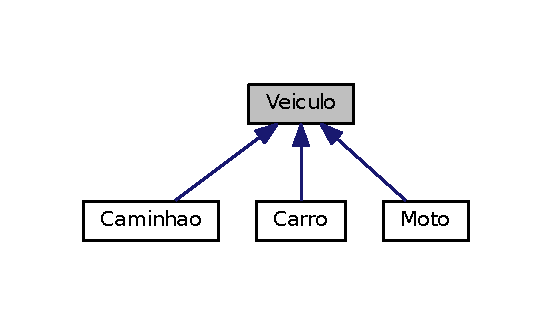
\includegraphics[width=265pt]{classVeiculo__inherit__graph}
\end{center}
\end{figure}


Collaboration diagram for Veiculo\+:\nopagebreak
\begin{figure}[H]
\begin{center}
\leavevmode
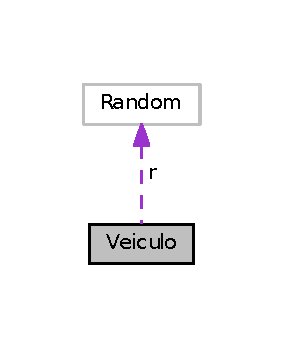
\includegraphics[width=136pt]{classVeiculo__coll__graph}
\end{center}
\end{figure}
\subsection*{Public Member Functions}
\begin{DoxyCompactItemize}
\item 
\hyperlink{classVeiculo_a9e42cc073f5ec6269187d23fbf9f811d}{Veiculo} ()
\begin{DoxyCompactList}\small\item\em Função random, utilizada para gerar posições aleatórias. \end{DoxyCompactList}\item 
\hyperlink{classVeiculo_aac421cbaf36de9c7483f6d59ffbfa9b6}{Veiculo} (int x, int y, int velocidade, String cor, boolean fabrica)
\item 
int \hyperlink{classVeiculo_a28cf763354cb7f3d14272c9e793db57e}{setX} ()
\item 
void \hyperlink{classVeiculo_a96a258d5c102f8e0c11d655e1992bdb2}{andaX} (int x)
\item 
void \hyperlink{classVeiculo_a3e63d6cddc5c6dea8302dc1c8e9f12bc}{andaY} (int y)
\item 
int \hyperlink{classVeiculo_ac0356427caf9839b90e558c99c09395f}{setY} ()
\item 
int \hyperlink{classVeiculo_a235b29e1e25ec8c769b20fb2aeba8404}{getX} ()
\item 
int \hyperlink{classVeiculo_a06b2a923e51186673a016f75d10363d3}{getY} ()
\item 
int \hyperlink{classVeiculo_a29ede179017c05f28aebf02922a5478b}{get\+Velocidade} ()
\item 
String \hyperlink{classVeiculo_ad1df848daf28895b13071d6dec374480}{get\+Cor} ()
\item 
void \hyperlink{classVeiculo_a8201bb998eb49364bb5d5bb05ce531ab}{set\+Fabrica} (boolean status)
\item 
boolean \hyperlink{classVeiculo_a6447f0eeb99399f1f96e835c22a88479}{get\+Fabrica} ()
\end{DoxyCompactItemize}


\subsection{Constructor \& Destructor Documentation}
\mbox{\Hypertarget{classVeiculo_a9e42cc073f5ec6269187d23fbf9f811d}\label{classVeiculo_a9e42cc073f5ec6269187d23fbf9f811d}} 
\index{Veiculo@{Veiculo}!Veiculo@{Veiculo}}
\index{Veiculo@{Veiculo}!Veiculo@{Veiculo}}
\subsubsection{\texorpdfstring{Veiculo()}{Veiculo()}\hspace{0.1cm}{\footnotesize\ttfamily [1/2]}}
{\footnotesize\ttfamily Veiculo.\+Veiculo (\begin{DoxyParamCaption}{ }\end{DoxyParamCaption})\hspace{0.3cm}{\ttfamily [inline]}}



Função random, utilizada para gerar posições aleatórias. 

Construtor da classe Veículo Incializa as váriaveis de veículo \mbox{\Hypertarget{classVeiculo_aac421cbaf36de9c7483f6d59ffbfa9b6}\label{classVeiculo_aac421cbaf36de9c7483f6d59ffbfa9b6}} 
\index{Veiculo@{Veiculo}!Veiculo@{Veiculo}}
\index{Veiculo@{Veiculo}!Veiculo@{Veiculo}}
\subsubsection{\texorpdfstring{Veiculo()}{Veiculo()}\hspace{0.1cm}{\footnotesize\ttfamily [2/2]}}
{\footnotesize\ttfamily Veiculo.\+Veiculo (\begin{DoxyParamCaption}\item[{int}]{x,  }\item[{int}]{y,  }\item[{int}]{velocidade,  }\item[{String}]{cor,  }\item[{boolean}]{fabrica }\end{DoxyParamCaption})\hspace{0.3cm}{\ttfamily [inline]}}

Construtor da classe Veículo Cria veículos com variáveis que são recebidas na chamada das funções de cada veículo específico


\begin{DoxyParams}{Parameters}
{\em x} & \\
\hline
{\em y} & \\
\hline
{\em velocidade} & \\
\hline
{\em cor} & \\
\hline
{\em fabrica} & \\
\hline
\end{DoxyParams}


\subsection{Member Function Documentation}
\mbox{\Hypertarget{classVeiculo_a96a258d5c102f8e0c11d655e1992bdb2}\label{classVeiculo_a96a258d5c102f8e0c11d655e1992bdb2}} 
\index{Veiculo@{Veiculo}!andaX@{andaX}}
\index{andaX@{andaX}!Veiculo@{Veiculo}}
\subsubsection{\texorpdfstring{anda\+X()}{andaX()}}
{\footnotesize\ttfamily void Veiculo.\+andaX (\begin{DoxyParamCaption}\item[{int}]{x }\end{DoxyParamCaption})\hspace{0.3cm}{\ttfamily [inline]}}

Altera o valor de X de um veículo com base no que será passado dentro de cada veículo específico


\begin{DoxyParams}{Parameters}
{\em x} & \\
\hline
\end{DoxyParams}
\mbox{\Hypertarget{classVeiculo_a3e63d6cddc5c6dea8302dc1c8e9f12bc}\label{classVeiculo_a3e63d6cddc5c6dea8302dc1c8e9f12bc}} 
\index{Veiculo@{Veiculo}!andaY@{andaY}}
\index{andaY@{andaY}!Veiculo@{Veiculo}}
\subsubsection{\texorpdfstring{anda\+Y()}{andaY()}}
{\footnotesize\ttfamily void Veiculo.\+andaY (\begin{DoxyParamCaption}\item[{int}]{y }\end{DoxyParamCaption})\hspace{0.3cm}{\ttfamily [inline]}}

Altera o valor de Y de um veículo com base no que será passado dentro de cada veículo específico


\begin{DoxyParams}{Parameters}
{\em y} & \\
\hline
\end{DoxyParams}
\mbox{\Hypertarget{classVeiculo_ad1df848daf28895b13071d6dec374480}\label{classVeiculo_ad1df848daf28895b13071d6dec374480}} 
\index{Veiculo@{Veiculo}!get\+Cor@{get\+Cor}}
\index{get\+Cor@{get\+Cor}!Veiculo@{Veiculo}}
\subsubsection{\texorpdfstring{get\+Cor()}{getCor()}}
{\footnotesize\ttfamily String Veiculo.\+get\+Cor (\begin{DoxyParamCaption}{ }\end{DoxyParamCaption})\hspace{0.3cm}{\ttfamily [inline]}}

\begin{DoxyReturn}{Returns}
A cor do veículo 
\end{DoxyReturn}
\mbox{\Hypertarget{classVeiculo_a6447f0eeb99399f1f96e835c22a88479}\label{classVeiculo_a6447f0eeb99399f1f96e835c22a88479}} 
\index{Veiculo@{Veiculo}!get\+Fabrica@{get\+Fabrica}}
\index{get\+Fabrica@{get\+Fabrica}!Veiculo@{Veiculo}}
\subsubsection{\texorpdfstring{get\+Fabrica()}{getFabrica()}}
{\footnotesize\ttfamily boolean Veiculo.\+get\+Fabrica (\begin{DoxyParamCaption}{ }\end{DoxyParamCaption})\hspace{0.3cm}{\ttfamily [inline]}}

\begin{DoxyReturn}{Returns}
Se um veículo está ou não em uma fábrica 
\end{DoxyReturn}
\mbox{\Hypertarget{classVeiculo_a29ede179017c05f28aebf02922a5478b}\label{classVeiculo_a29ede179017c05f28aebf02922a5478b}} 
\index{Veiculo@{Veiculo}!get\+Velocidade@{get\+Velocidade}}
\index{get\+Velocidade@{get\+Velocidade}!Veiculo@{Veiculo}}
\subsubsection{\texorpdfstring{get\+Velocidade()}{getVelocidade()}}
{\footnotesize\ttfamily int Veiculo.\+get\+Velocidade (\begin{DoxyParamCaption}{ }\end{DoxyParamCaption})\hspace{0.3cm}{\ttfamily [inline]}}

\begin{DoxyReturn}{Returns}
A velocidade do veículo 
\end{DoxyReturn}
\mbox{\Hypertarget{classVeiculo_a235b29e1e25ec8c769b20fb2aeba8404}\label{classVeiculo_a235b29e1e25ec8c769b20fb2aeba8404}} 
\index{Veiculo@{Veiculo}!getX@{getX}}
\index{getX@{getX}!Veiculo@{Veiculo}}
\subsubsection{\texorpdfstring{get\+X()}{getX()}}
{\footnotesize\ttfamily int Veiculo.\+getX (\begin{DoxyParamCaption}{ }\end{DoxyParamCaption})\hspace{0.3cm}{\ttfamily [inline]}}

\begin{DoxyReturn}{Returns}
O valor de X do veículo 
\end{DoxyReturn}
\mbox{\Hypertarget{classVeiculo_a06b2a923e51186673a016f75d10363d3}\label{classVeiculo_a06b2a923e51186673a016f75d10363d3}} 
\index{Veiculo@{Veiculo}!getY@{getY}}
\index{getY@{getY}!Veiculo@{Veiculo}}
\subsubsection{\texorpdfstring{get\+Y()}{getY()}}
{\footnotesize\ttfamily int Veiculo.\+getY (\begin{DoxyParamCaption}{ }\end{DoxyParamCaption})\hspace{0.3cm}{\ttfamily [inline]}}

\begin{DoxyReturn}{Returns}
O valor de Y do veículo 
\end{DoxyReturn}
\mbox{\Hypertarget{classVeiculo_a8201bb998eb49364bb5d5bb05ce531ab}\label{classVeiculo_a8201bb998eb49364bb5d5bb05ce531ab}} 
\index{Veiculo@{Veiculo}!set\+Fabrica@{set\+Fabrica}}
\index{set\+Fabrica@{set\+Fabrica}!Veiculo@{Veiculo}}
\subsubsection{\texorpdfstring{set\+Fabrica()}{setFabrica()}}
{\footnotesize\ttfamily void Veiculo.\+set\+Fabrica (\begin{DoxyParamCaption}\item[{boolean}]{status }\end{DoxyParamCaption})\hspace{0.3cm}{\ttfamily [inline]}}

Define se um veículo está ou não dentro de uma fábrica, com base no que é recebido em status


\begin{DoxyParams}{Parameters}
{\em status} & \\
\hline
\end{DoxyParams}
\mbox{\Hypertarget{classVeiculo_a28cf763354cb7f3d14272c9e793db57e}\label{classVeiculo_a28cf763354cb7f3d14272c9e793db57e}} 
\index{Veiculo@{Veiculo}!setX@{setX}}
\index{setX@{setX}!Veiculo@{Veiculo}}
\subsubsection{\texorpdfstring{set\+X()}{setX()}}
{\footnotesize\ttfamily int Veiculo.\+setX (\begin{DoxyParamCaption}{ }\end{DoxyParamCaption})\hspace{0.3cm}{\ttfamily [inline]}}

Cria um valor aleatório para o X do veículo

\begin{DoxyReturn}{Returns}
O valor aleatório gerado para X 
\end{DoxyReturn}
\mbox{\Hypertarget{classVeiculo_ac0356427caf9839b90e558c99c09395f}\label{classVeiculo_ac0356427caf9839b90e558c99c09395f}} 
\index{Veiculo@{Veiculo}!setY@{setY}}
\index{setY@{setY}!Veiculo@{Veiculo}}
\subsubsection{\texorpdfstring{set\+Y()}{setY()}}
{\footnotesize\ttfamily int Veiculo.\+setY (\begin{DoxyParamCaption}{ }\end{DoxyParamCaption})\hspace{0.3cm}{\ttfamily [inline]}}

Cria um valor aleatório para o Y do veículo

\begin{DoxyReturn}{Returns}
O valor aleatório gerado para Y 
\end{DoxyReturn}


The documentation for this class was generated from the following file\+:\begin{DoxyCompactItemize}
\item 
Veiculo.\+java\end{DoxyCompactItemize}

%--- End generated contents ---

% Index
\backmatter
\newpage
\phantomsection
\clearemptydoublepage
\addcontentsline{toc}{chapter}{Index}
\printindex

\end{document}
